\documentclass[12pt,letterpaper]{article}
\usepackage{graphicx,textcomp}
\usepackage{natbib}
\usepackage{setspace}
\usepackage{fullpage}
\usepackage{color}
\usepackage[reqno]{amsmath}
\usepackage{amsthm}
\usepackage{fancyvrb}
\usepackage{amssymb,enumerate}
\usepackage[all]{xy}
\usepackage{endnotes}
\usepackage{lscape}
\newtheorem{com}{Comment}
\usepackage{float}
\usepackage{hyperref}
\newtheorem{lem} {Lemma}
\newtheorem{prop}{Proposition}
\newtheorem{thm}{Theorem}
\newtheorem{defn}{Definition}
\newtheorem{cor}{Corollary}
\newtheorem{obs}{Observation}
\usepackage[compact]{titlesec}
\usepackage{dcolumn}
\usepackage{tikz}
\usetikzlibrary{arrows}
\usepackage{multirow}
\usepackage{xcolor}
\newcolumntype{.}{D{.}{.}{-1}}
\newcolumntype{d}[1]{D{.}{.}{#1}}
\definecolor{light-gray}{gray}{0.65}
\usepackage{url}
\usepackage{listings}
\usepackage{color}
\definecolor{codegreen}{rgb}{0,0.6,0}
\definecolor{codegray}{rgb}{0.5,0.5,0.5}
\definecolor{codepurple}{rgb}{0.58,0,0.82}
\definecolor{backcolour}{rgb}{0.95,0.95,0.92}

\lstdefinestyle{mystyle}{
	backgroundcolor=\color{backcolour},   
	commentstyle=\color{codegreen},
	keywordstyle=\color{magenta},
	numberstyle=\tiny\color{codegray},
	stringstyle=\color{codepurple},
	basicstyle=\footnotesize,
	breakatwhitespace=false,         
	breaklines=true,                 
	captionpos=b,                    
	keepspaces=true,                 
	numbers=left,                    
	numbersep=5pt,                  
	showspaces=false,                
	showstringspaces=false,
	showtabs=false,                  
	tabsize=2
}
\lstset{style=mystyle}
\newcommand{\Sref}[1]{Section~\ref{#1}}
\newtheorem{hyp}{Hypothesis}

\title{Problem Set 2}
\date{Due: February 4, 2026}
\author{Data Visualisation for Social Scientists}

\begin{document}
	\maketitle
	
	\section*{Instructions}
	\begin{itemize}
	\item Please show your work! You may lose points by simply writing in the answer. If the problem requires you to execute commands in \texttt{R}, please include the code you used to get your answers. Please also include the \texttt{.R} file that contains your code. If you are not sure if work needs to be shown for a particular problem, please ask.
\item Your homework should be submitted electronically on GitHub.
\item This problem set is due before 23:59 on Wednesday February 4, 2026. No late assignments will be accepted.
	\end{itemize}
	
	\vspace{.25cm}
	\section*{Study of Religious Congregations in Switzerland}
	
The data for this problem set come from the	National Congregations Study Switzerland (NCSS), which was conducted in 2008–2009 and 2022–2023. The data provide information on organisational structure, staffing, finances, worship practices, youth and educational activities, social composition, external engagement, and inclusion norms. The data were collected using stratified random samples of congregations drawn from comprehensive censuses, with interviews completed by a single knowledgeable key informant in each congregation, most often the spiritual leader.

\subsection*{Data Manipulation}

\begin{enumerate}
\item Load the NCSS .csv file from \href{https://raw.githubusercontent.com/ASDS-TCD/DataViz_2026/refs/heads/main/datasets/NCSS_v1.csv}{GitHub} into your global environment. Use the select() function to keep these variables in your dataframe:

\lstinputlisting[language=R, firstline=26, lastline=29]{problem2.R} 

	\textit {I loaded the data into R as a csv file and isolated the key variables that are needed for the analysis.}
\begin{itemize}
	\item Congregation ID (\texttt{CASEID})
	\item Year (\texttt{YEAR})
	\item Region (\texttt{GDREGION})
	\item Number of official members (\texttt{NUMOFFMBR})
	\item 6-level religious classification (\texttt{TRAD6})
	\item 12-level religious classification (\texttt{TRAD12})
	\item Total income in last fiscal year (\texttt{INCOME})
\end{itemize}
\item Filter the dataset so that you only include Christian, Jewish, and Muslim congregations (Chrétiennes, Juives, Musulmanes) using the \texttt{TRAD6} variable.
\lstinputlisting[language=R, firstline=30, lastline=33]{problem2.R} 

	\textit {Filtered the dataset so that only the three religions are shown in the TRAD6 }
	\begin{verbatim}
		  CASEID YEAR          GDREGION NUMOFFMBR       TRAD6
		1    814 2022 Espace Mittelland      1300 Chrétiennes
		2   5171 2022  Région lémanique        NA Chrétiennes
		3   3755 2022 Espace Mittelland       575 Chrétiennes
		4   4636 2022            Zürich      2500 Chrétiennes
		5   1331 2022 Espace Mittelland        NA Chrétiennes
		6   4267 2022 Espace Mittelland      2000 Chrétiennes
		TRAD12 INCOME
		1        Protestantes réformées     NA
		2          Catholiques romaines     NA
		3          Catholiques romaines     NA
		4          Catholiques romaines     NA
		5 Évangéliques (conservatrices)     NA
		6          Catholiques romaines     NA
		> table(Religion$TRAD6)
		
		Chrétiennes      Juives  Musulmanes 
		1974          31         106
	\end{verbatim}
	
\item Compute for the number of congregations by religious classification (\texttt{TRAD6}) in each year, as well as the mean and median total income in last fiscal year (\texttt{INCOME}) by religious classification and year.

\lstinputlisting[language=R, firstline=34, lastline=50]{problem2.R} 

	\textit {I computed the number of congregations by religious classification in TRAD6 by year and then the mean and median income for the last fiscal year and dropped the NAs.}
	
		\begin{verbatim}
	YEAR TRAD6       total_members
	<int> <chr>               <dbl>
	1  2009 Chrétiennes            0 
	2  2009 Juives                 0 
	3  2009 Musulmanes             0 
	4  2022 Chrétiennes      1448291.
	5  2022 Juives             35083 
	6  2022 Musulmanes          7433
	
	 Income_last_year
	# A tibble: 3 × 4
	TRAD6       mean_income median_income count
	<chr>             <dbl>         <dbl> <int>
	1 Chrétiennes     474601.        201000   676
	2 Juives         2332500         115000     4
	3 Musulmanes       77941.         42500    17
	\end{verbatim}
	
	
\item Create a categorical variable for called \texttt{AVG\_INCOME} that is binary in which 1 = "Above average or average income" and 0 = "Below average income", which indicates if a congregation is $\geq$ average income or $<$ average income among congregations that year.

\lstinputlisting[language=R, firstline=51, lastline=59]{problem2.R} 

	\textit {I created code to see if the income of a congregation is average income 
		 or above average income based on other congregations.} 
		
\end{enumerate}

\subsection*{Data Visualization}

\begin{enumerate}
	\item Create a bar plot visualizing the proportion of congregations above and below the average income (\texttt{AVG\_INCOME}) in each year by 12-level religious classification (\texttt{TRAD12}). Hint: Use \texttt{facet()} for \texttt{YEAR}.
	
	\lstinputlisting[language=R, firstline=61, lastline=84]{problem2.R} 
	
		\textit {I created a bar plot showing the proportion of congregations above and below the average income}
		
		\begin{center}
			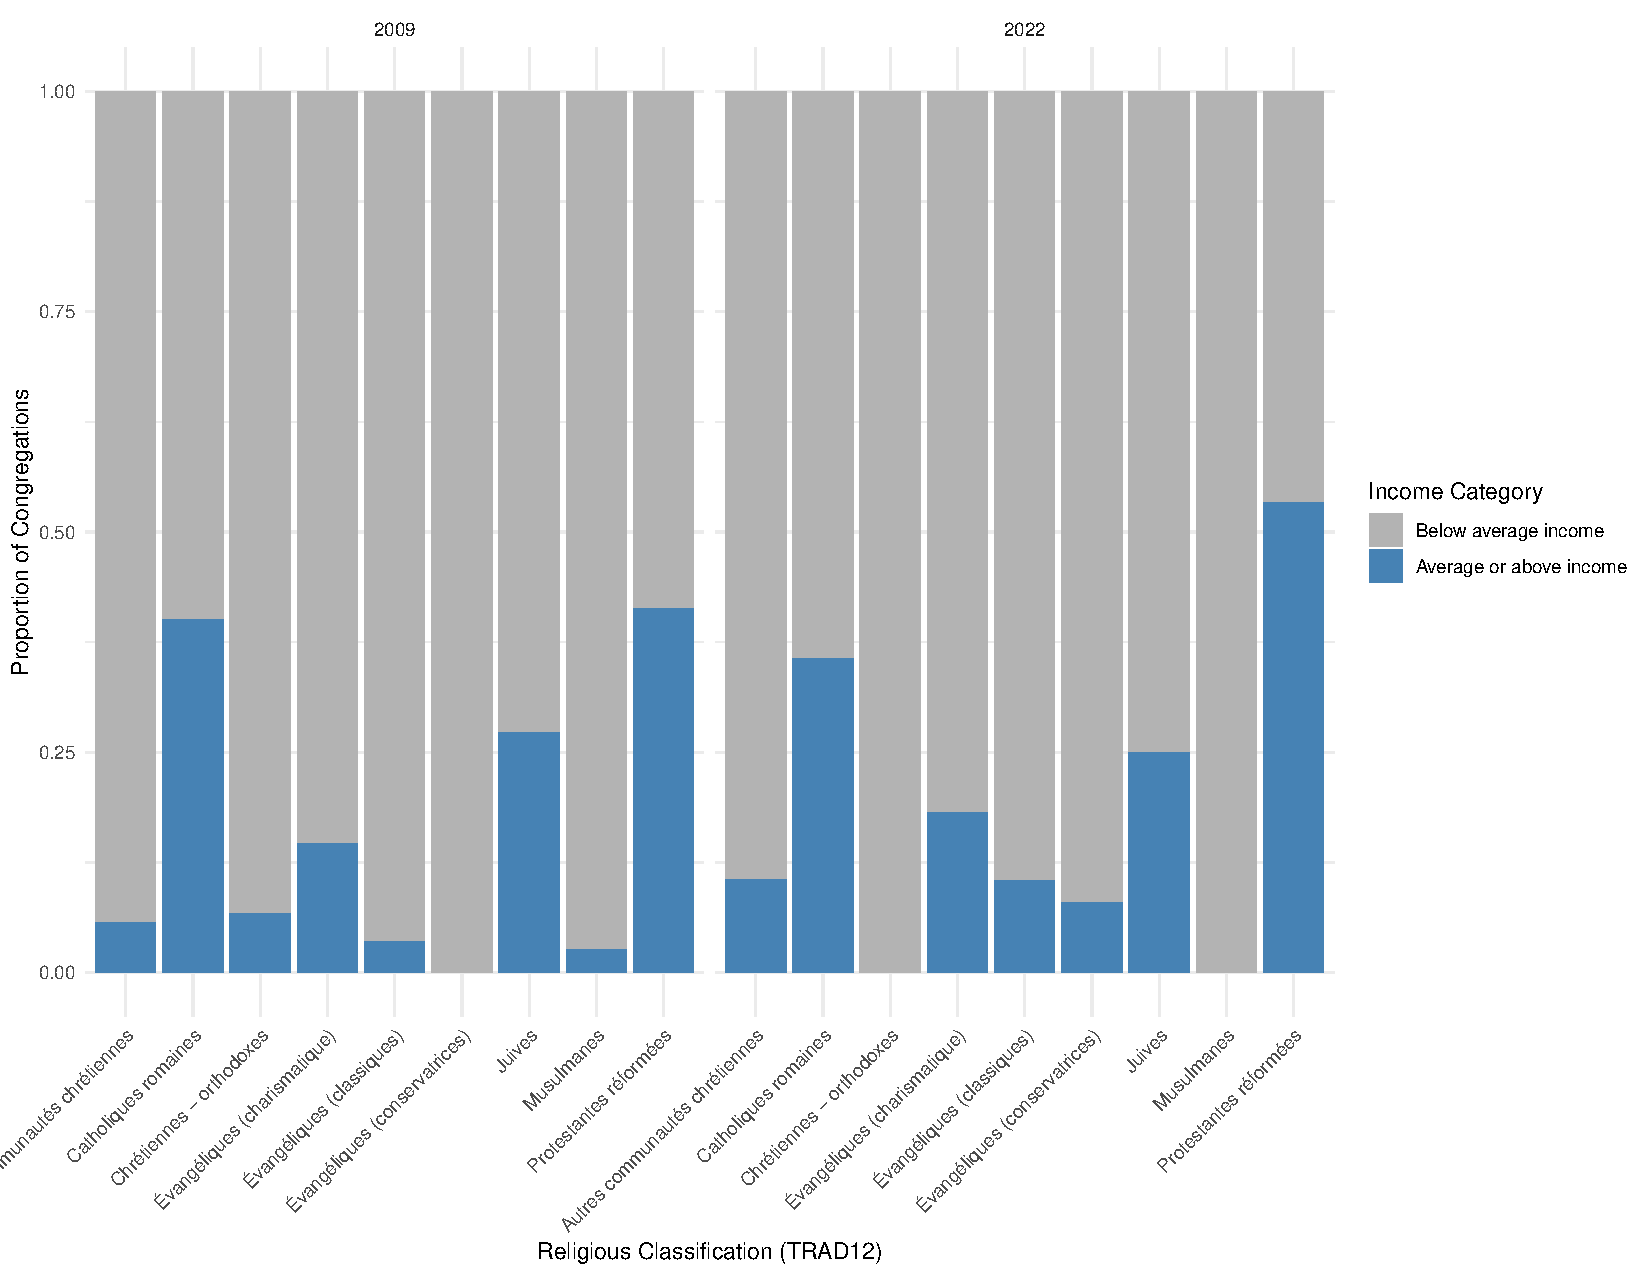
\includegraphics[width=0.7\textwidth]{religion_graph1.pdf}
		\end{center}
		
	\item Make a histogram using \texttt{geom\_col()} detailing the number of official members using the 12-level religious classification (\texttt{TRAD12}) distinguishing between the 6-level religious classification (\texttt{TRAD6}) in 2022. Hint: Use \texttt{facet()} for \texttt{TRAD6}, with \texttt{TRAD12} on the x-axis in addition to group/fill with the \texttt{position="dodge"}.
	
	\lstinputlisting[language=R, firstline=93, lastline=113]{problem2.R} 
	
		\textit {I made a histogram for the number of official members by religious classification}
		
		\begin{center}
			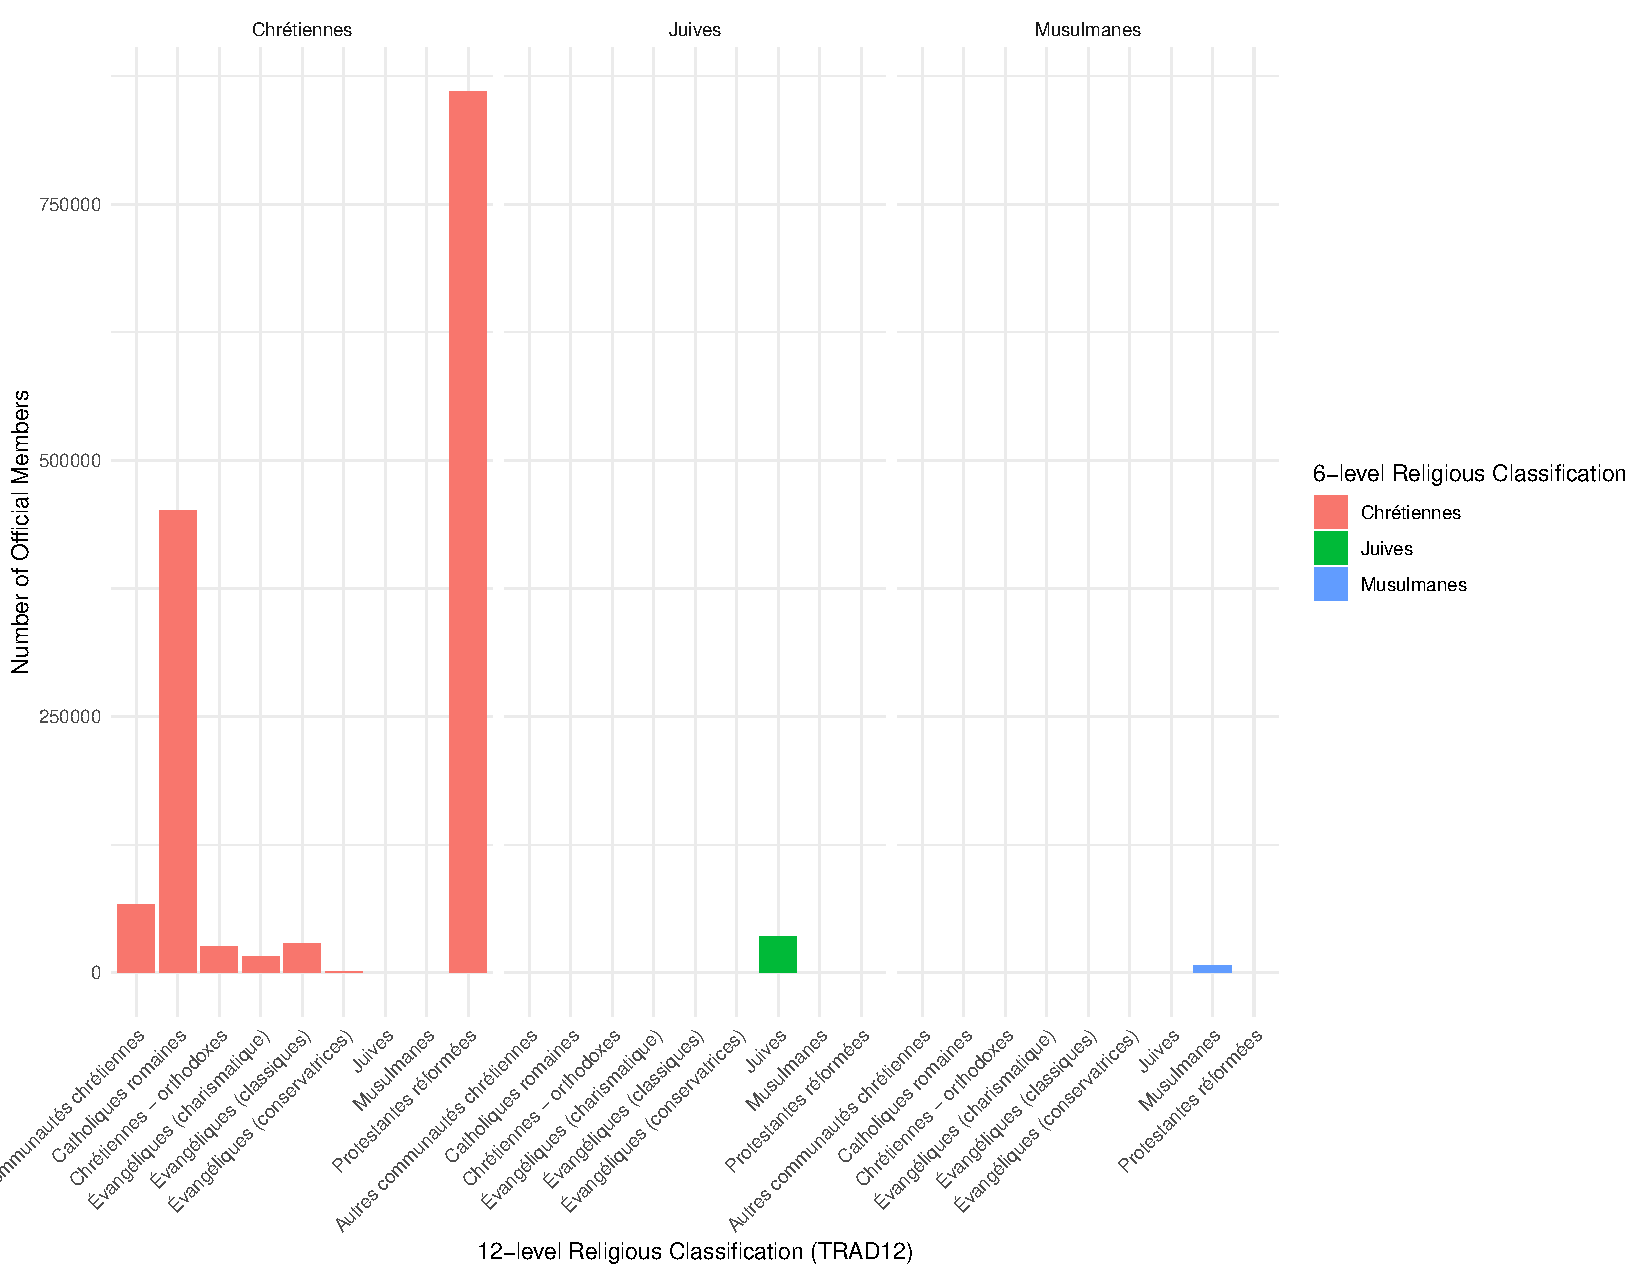
\includegraphics[width=0.7\textwidth]{religion_graph2.pdf}
		\end{center}
		
	\item Display the distribution of yearly income (\texttt{INCOME}) in 2022 for congregations in each region (\texttt{GDREGION}) using ridge plots.
	
	\lstinputlisting[language=R, firstline=120, lastline=138]{problem2.R} 
	
		\textit {I created a ridge plot to display the distribution of yearly income in 2022 for congregations in each region. }
		
		\begin{center}
			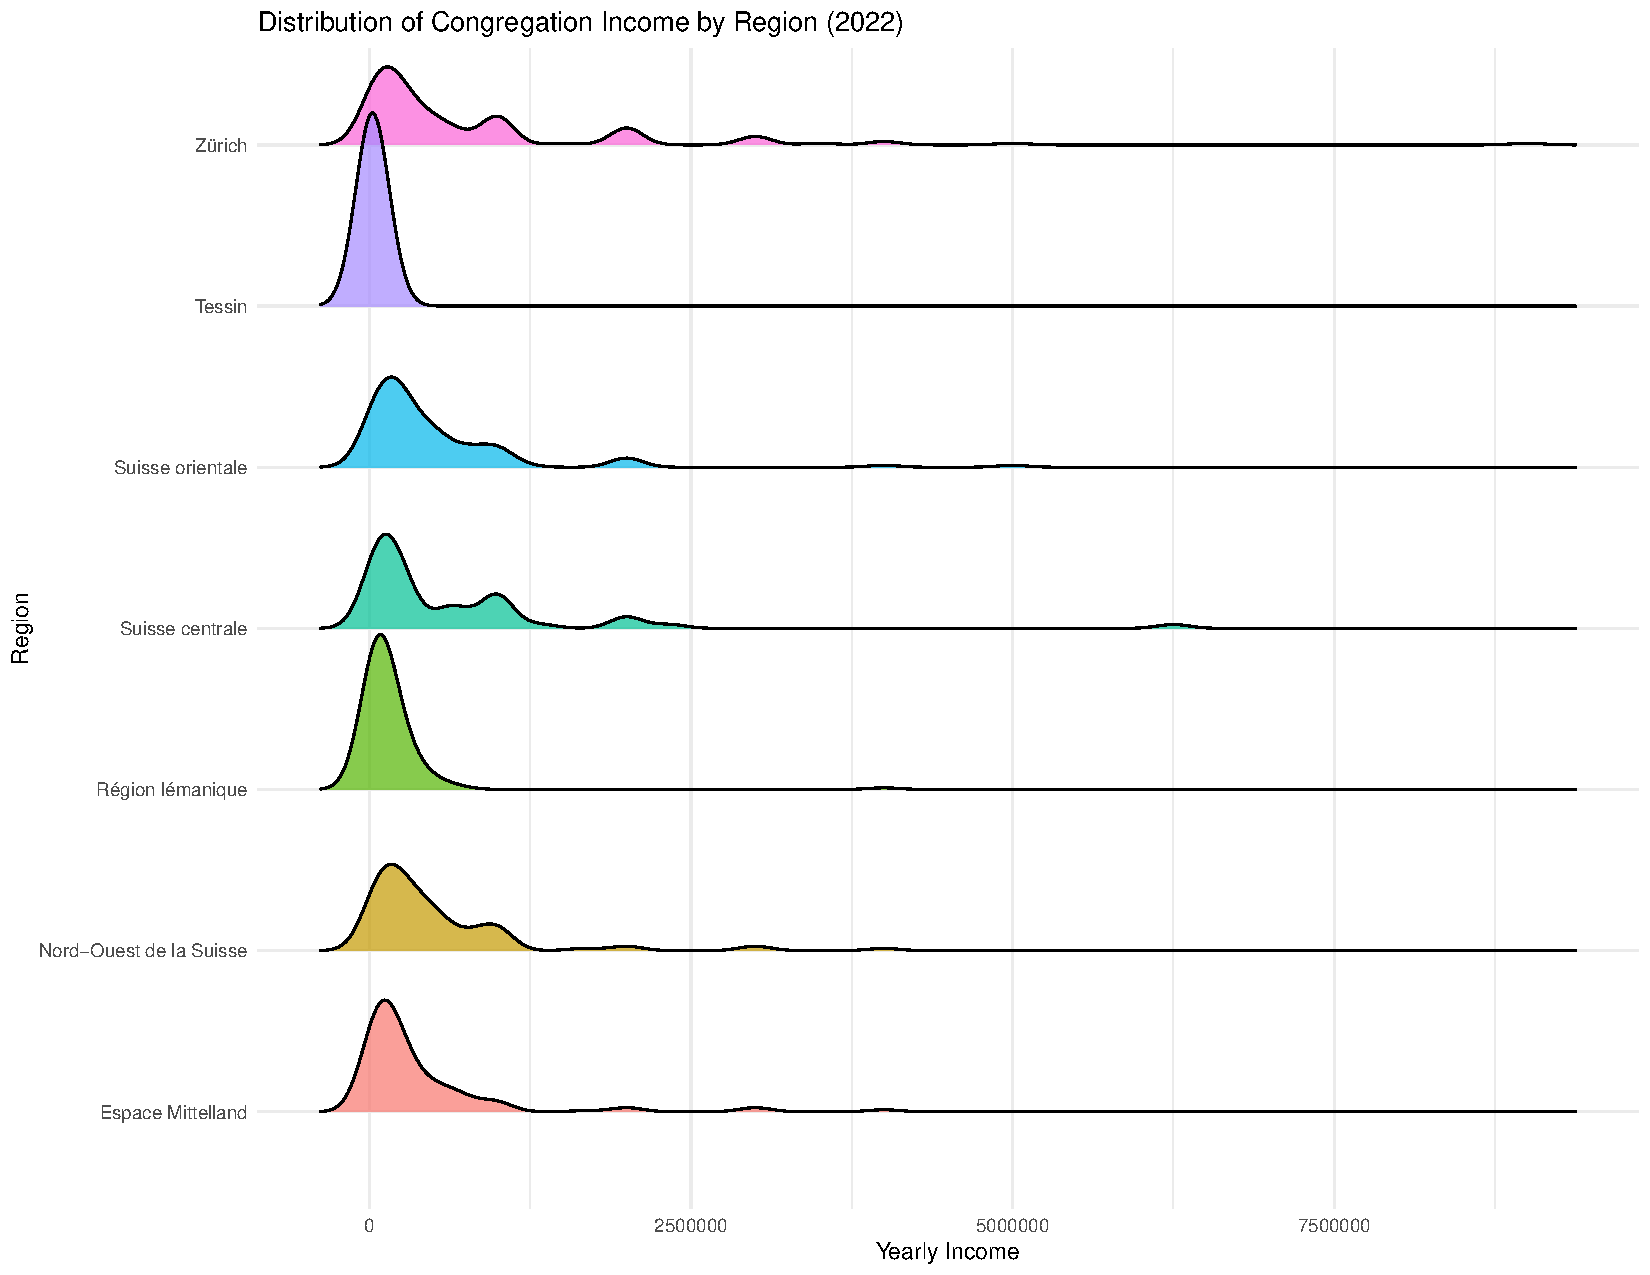
\includegraphics[width=0.7\textwidth]{religion_graph3.pdf}
		\end{center}
		
	\item Create a boxplot of the number of official members per congregation in 2022 by religious classification (\texttt{TRAD6}) and region (\texttt{GDREGION}). Hint: Use \texttt{facet()} for \texttt{GDREGION}.
	
	\lstinputlisting[language=R, firstline=145, lastline=165]{problem2.R} 
	
		\textit {I created a boxplot for the members per congregation in 2022 by religious classification}
		\begin{center}
			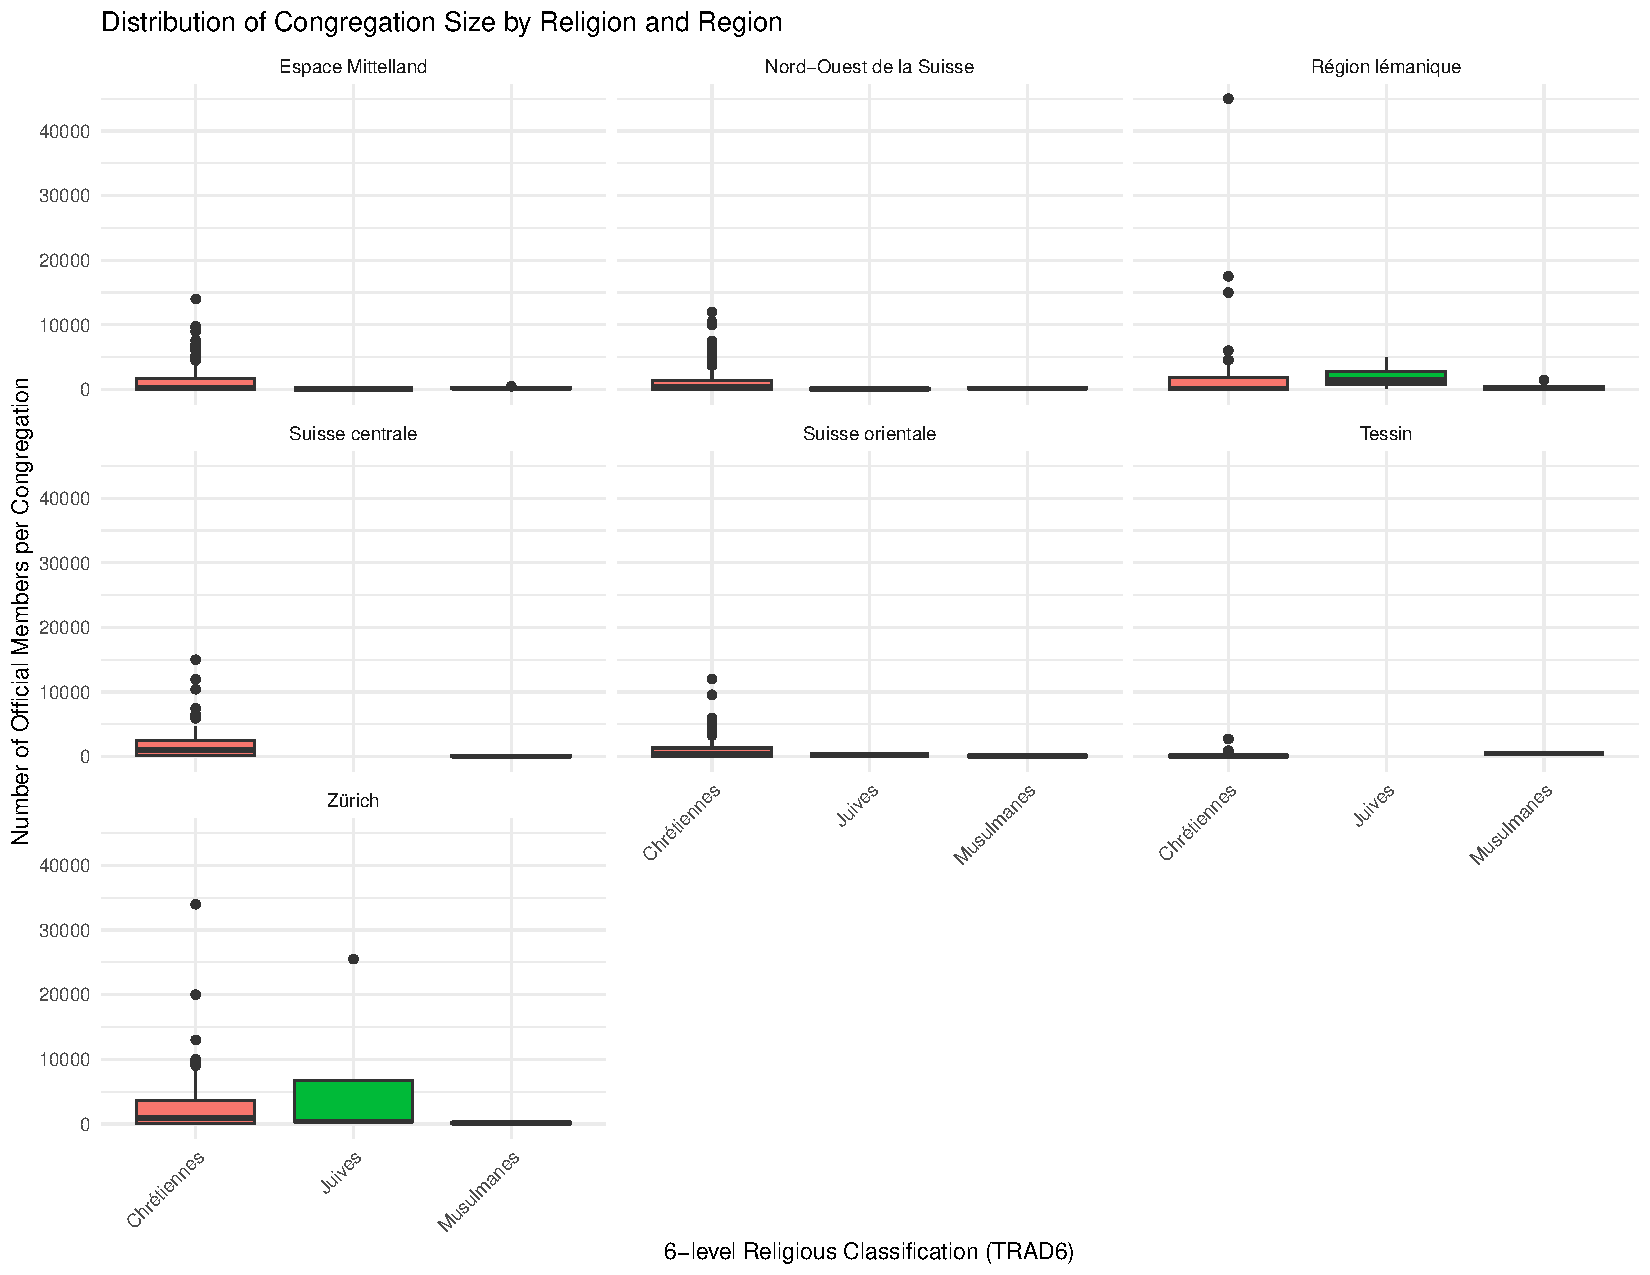
\includegraphics[width=0.7\textwidth]{religion_graph4.pdf}
		\end{center}

\end{enumerate}


\end{document}
